\subsubsection{Home}
Pagina di ``benvenuto'' della WebApp, presenta due sezioni:
\begin{itemize}
\item Resoconto delle ultime 4 anomalie riscontrate, organizzate in
  una lista
  \begin{figure}[ht]
    \centering
    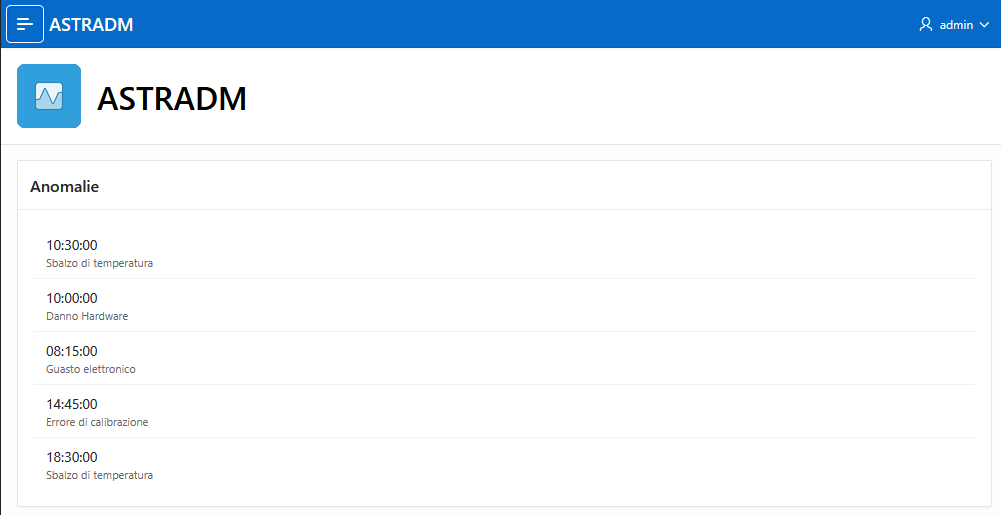
\includegraphics[width=\linewidth]{images/home-anomalie.png}
    \caption{Resoconto delle ultime 4 anomalie}
    \label{fig:anomalie}
  \end{figure}
\item Grafico a torta sullo stato dei sensori
  \begin{figure}[ht]
    \centering
    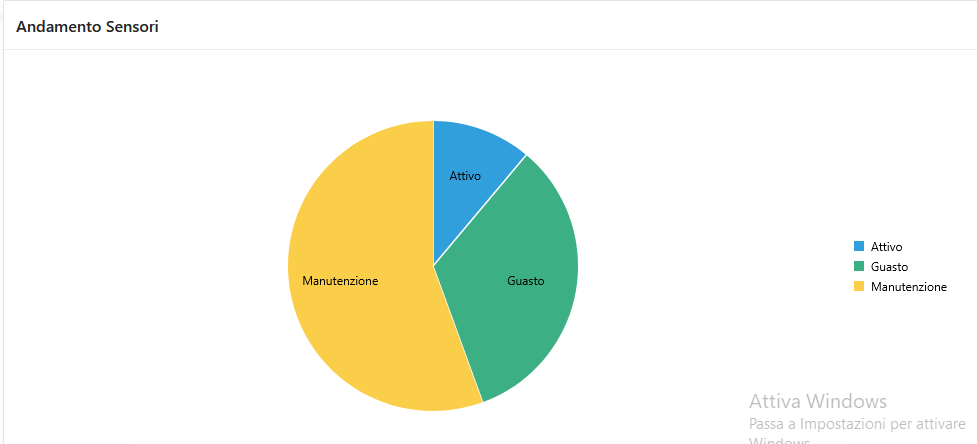
\includegraphics[width=\linewidth]{images/home-sensori.png}
    \caption{Grafico rappresentante lo stato dei sensori}
    \label{fig:sensori}
  \end{figure}
\end{itemize}
%%% Local Variables:
%%% mode: LaTeX
%%% TeX-master: "Tesina"
%%% End:
